\chapter{Bagaimana Hewan Menjadi Dewasa}\label{ch:g2:animals-grow-up}

Seekor anak kucing sudah tampak seperti kucing kecil sejak hari
pertamanya. Tetapi katak di kolam bermula sebagai \omterm{ex:g2:animals-grow-up:frog}{berudu} berbentuk
ikan tanpa kaki, dan kupu-kupu di semak buddleia menghabiskan
berminggu-minggu sebagai \omterm{ex:g2:animals-grow-up:butterfly}{ulat} yang merayap. \omterm{def:g1:animals-around-us:animal}{Hewan} muda tidak semuanya
menyerupai induknya --- sebagian harus berubah bentuk sama sekali
dalam perjalanan menuju dewasa.

\section{Dari telur atau lahir hidup}

\begin{definition}[Dua cara dilahirkan]\label{def:g2:animals-grow-up:born}
\omterm{def:g1:animals-around-us:animal}{Hewan} muda datang ke dunia dengan dua cara:
\begin{itemize}
  \item kebanyakan menetas dari sebutir \emph{telur}\index{telur} yang
        dikeluarkan induknya: burung, ikan, katak, siput, serangga;
  \item lainnya \emph{lahir hidup}\index{lahir hidup}, keluar dari
        tubuh induknya dalam keadaan sudah terbentuk, lalu meminum
        \emph{susu}\index{susu} induknya: kucing, anjing, sapi,
        kelinci --- dan manusia.
\end{itemize}
\end{definition}

\begin{example}[Di kandang ayam dan keranjang]\label{ex:g2:animals-grow-up:henhouse}
Ayam betina mengeluarkan \omterm{def:g2:animals-grow-up:born}{telur} lalu mengeraminya agar tetap hangat;
sesudah tiga minggu, anak-anak ayam memecahkan \omterm{def:g1:animals-around-us:covering}{cangkang} dan menetas.
Di keranjang dekat tungku, anak-anak kucing \omterm{def:g2:animals-grow-up:born}{lahir hidup} pada malam
yang sama, dan dalam waktu satu jam mereka sudah menemukan \omterm{def:g2:animals-grow-up:born}{susu}
induknya.
\end{example}

\begin{remark}[Telur bukan batu]\label{rem:g2:animals-grow-up:egg}
Di dalam \omterm{def:g2:animals-grow-up:born}{telur} yang dierami, seekor anak ayam sedang dibangun dengan
diam, diberi makan oleh kuning telurnya. \omterm{def:g2:animals-grow-up:born}{Telurnya} tidak sedang
menunggu --- ia sedang bekerja. Itulah sebabnya ayam betina menjaga
\omterm{def:g2:animals-grow-up:born}{telurnya} tetap hangat, dan sebabnya \omterm{def:g2:animals-grow-up:born}{telur} dari lemari es, yang memang
tidak akan menetas, tidak boleh dipersalahkan pada dinginnya.
\end{remark}

\section{Tumbuh tanpa berubah bentuk}

\begin{definition}[Tumbuh serupa induknya]\label{def:g2:animals-grow-up:direct}
Banyak \omterm{def:g1:animals-around-us:animal}{hewan} muda merupakan \emph{tiruan kecil
induknya}\index{tiruan kecil induk}: anak kucing adalah kucing kecil,
anak kuda adalah kuda kecil, anak ayam adalah ayam kecil. Menjadi
dewasa, bagi mereka, berarti bertambah besar dan bertambah kuat ---
bentuk tubuhnya tetap sama.
\end{definition}

\begin{example}[Anak kucing menjadi kucing]\label{ex:g2:animals-grow-up:kitten}
Anak kucing yang baru lahir meminum \omterm{def:g2:animals-grow-up:born}{susu} dengan \omterm{def:g1:the-five-senses:sense}{mata} terpejam. Pada
umur satu bulan ia bermain dan menerkam; pada umur enam bulan ia
berburu seperti kucing dewasa; pada umur satu tahun ia sudah dewasa,
barangkali dengan anak-anaknya sendiri. Kucing kecil, kucing yang
lebih besar, kucing: bentuk yang sama sepanjang jalannya.
\end{example}

\section{Tumbuh dengan berubah bentuk}

\begin{definition}[Metamorfosis]\label{def:g2:animals-grow-up:metamorphosis}
Sebagian \omterm{def:g1:animals-around-us:animal}{hewan} muda sama sekali tidak mirip induknya, dan harus
mengubah seluruh bentuk tubuhnya untuk menjadi dewasa. Perubahan besar
itu disebut \emph{metamorfosis}\index{metamorfosis}. \omterm{ex:g2:animals-grow-up:frog}{Berudu} menjadi
katak; \omterm{ex:g2:animals-grow-up:butterfly}{ulat} menjadi kupu-kupu.
\end{definition}

\begin{example}[Jalan hidup katak]\label{ex:g2:animals-grow-up:frog}
Dari \omterm{def:g2:animals-grow-up:born}{telur} katak di kolam menetaslah \emph{berudu}\index{berudu}:
berkepala bulat, berekor panjang, tanpa kaki, bernapas di dalam air
seperti ikan. Lalu, minggu demi minggu: kaki belakang muncul, kemudian
kaki depan; ekornya menyusut hilang; dan pada suatu hari seekor katak
kecil memanjat ke tepian. \omterm{def:g1:animals-around-us:animal}{Hewan} yang sama --- dibangun ulang.
\end{example}

\begin{omfigure}
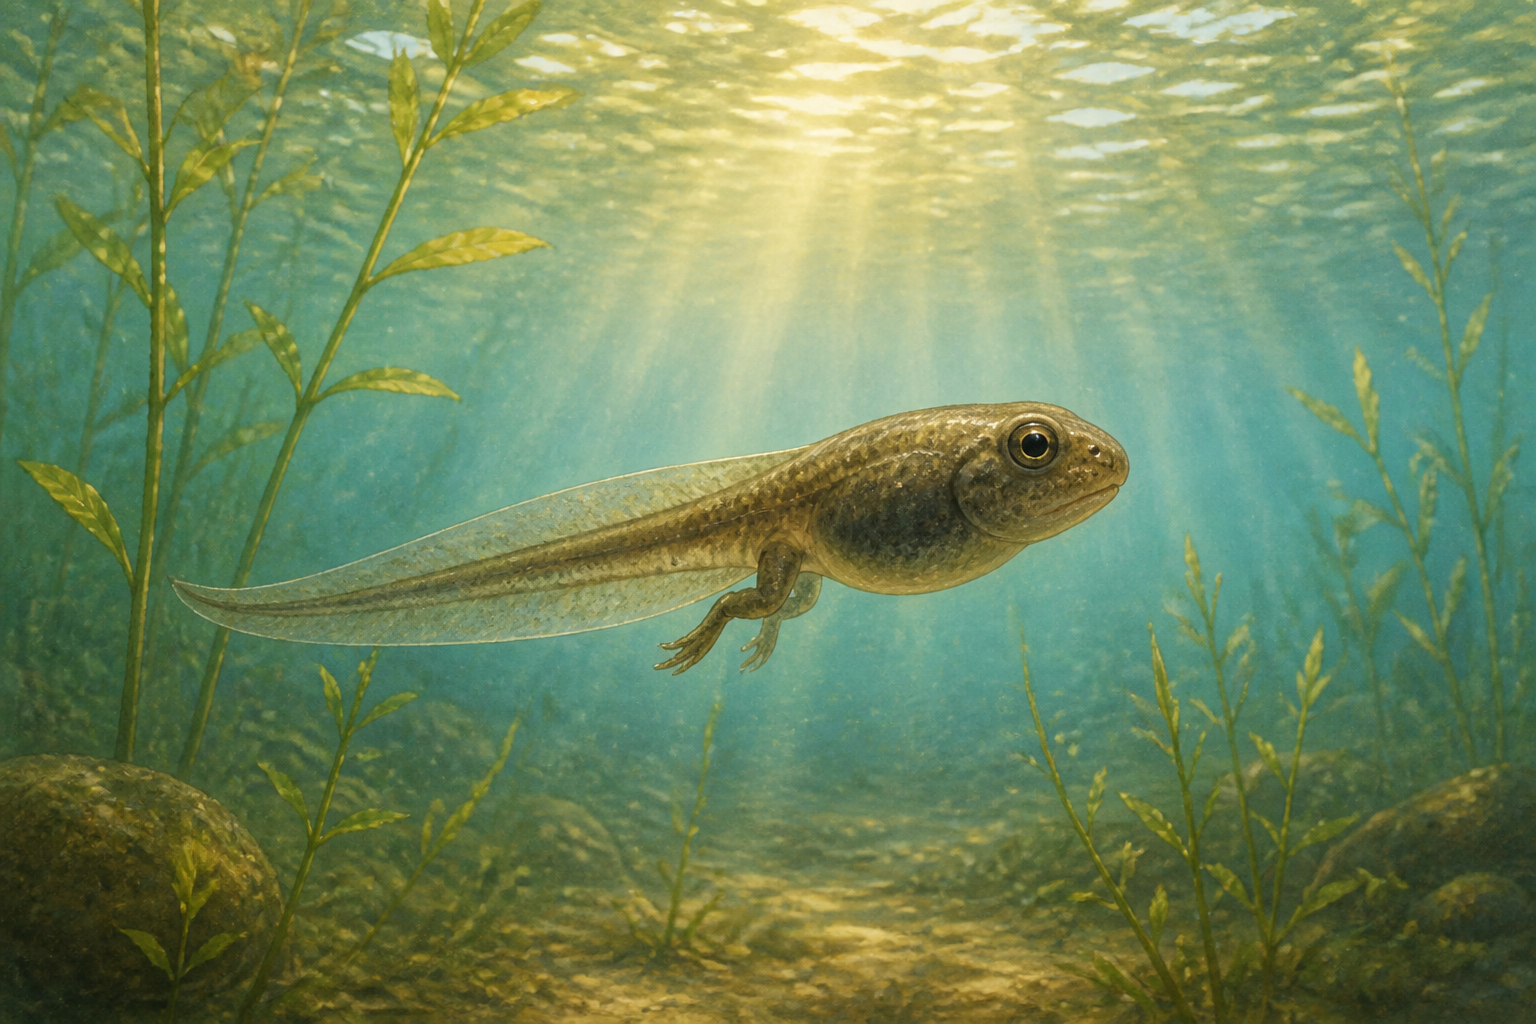
\includegraphics[width=0.6\linewidth]{images/book1/ai/g2-grow-tadpole.png}

{\small Tertangkap di tengah \omterm{def:g2:animals-grow-up:metamorphosis}{metamorfosis}: kaki belakang sudah tumbuh,
kaki depan belum datang, ekornya masih panjang.}
\end{omfigure}

\begin{omfigure}
\begin{tikzpicture}
  \node[anchor=south west, inner sep=0] (img) at (0,0)
    {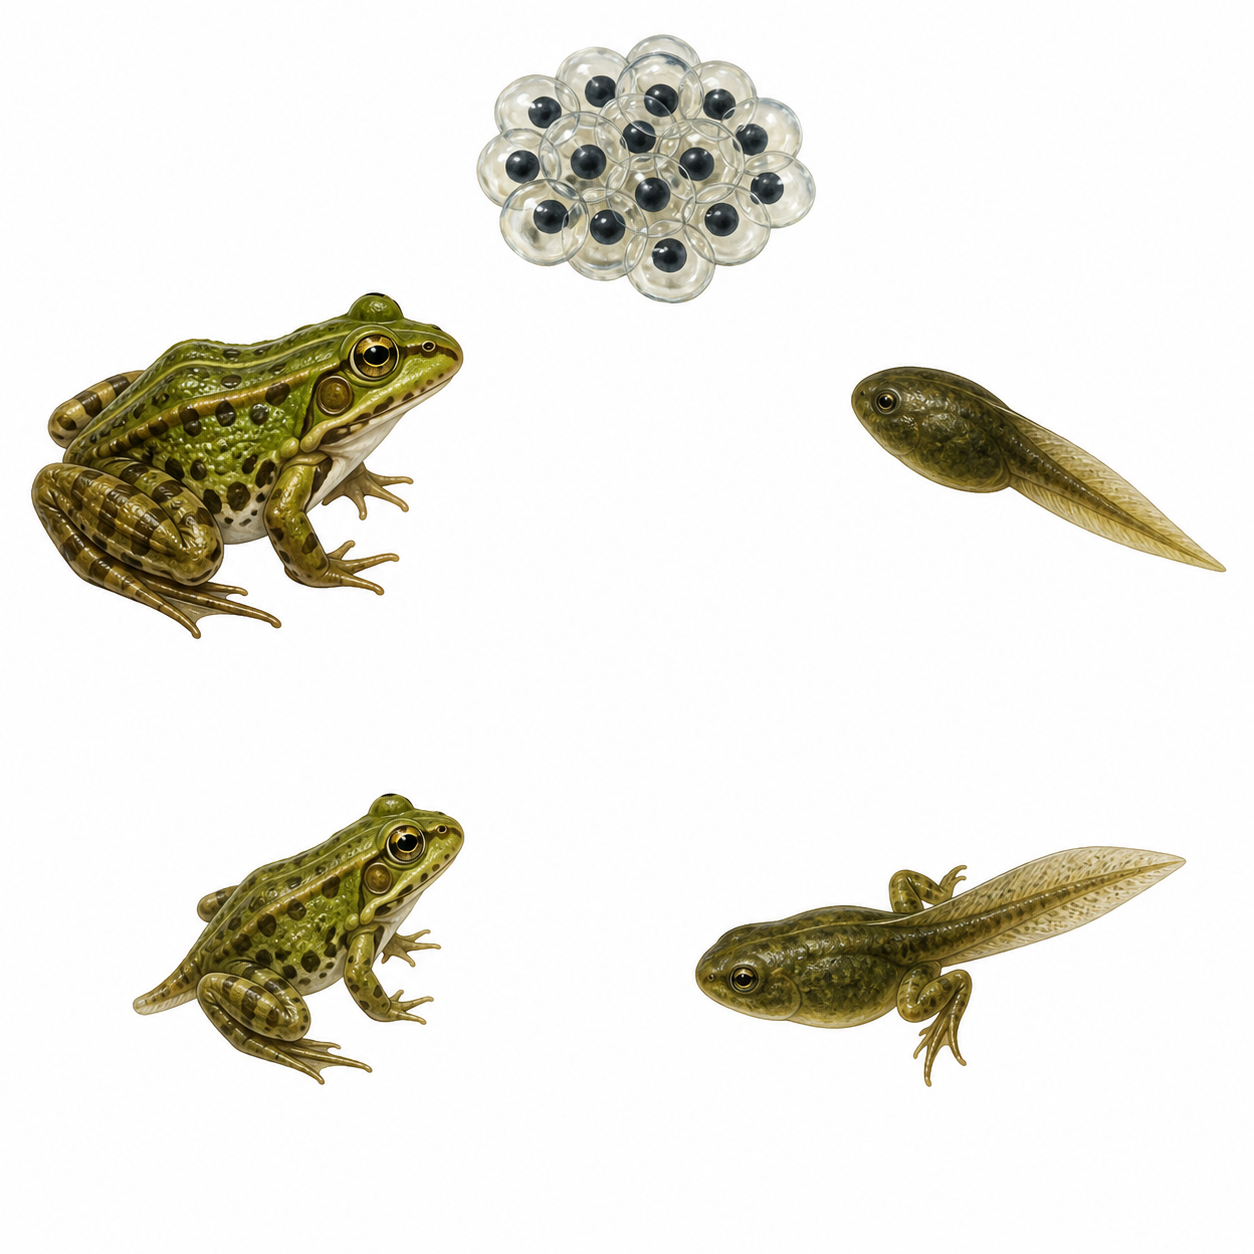
\includegraphics[width=0.72\linewidth]{images/book1/ai/fig-frog-cycle.png}};
  \begin{scope}[x={(img.south east)}, y={(img.north west)},
      every node/.style={font=\small}]
    \node[above] at (0.33,0.92) {telur di kolam};
    \node[right, align=left] at (0.87,0.44)
      {berudu:\\ berekor, tanpa kaki};
    \node[below, align=center] at (0.80,0.05)
      {kaki belakang tumbuh,\\ lalu kaki depan};
    \node[below] at (0.22,0.05) {ekornya menyusut: katak kecil};
    \node[left, align=right] at (0.075,0.78) {katak dewasa};
    \draw[->, thick, omProp] (0.70,0.86) to[bend left=20] (0.87,0.68);
    \draw[->, thick, omProp] (0.88,0.38) to[bend left=15] (0.85,0.25);
    \draw[->, thick, omProp] (0.60,0.16) to[bend left=12] (0.42,0.14);
    \draw[->, thick, omProp] (0.16,0.32) to[bend left=15] (0.13,0.48);
    \draw[->, thick, omProp] (0.30,0.80) to[bend left=18] (0.42,0.88);
  \end{scope}
\end{tikzpicture}

{\small \omterm{def:g2:animals-grow-up:metamorphosis}{Metamorfosis} katak, berputar searah jarum jam mulai dari
\omterm{def:g2:animals-grow-up:born}{telurnya}: \omterm{ex:g2:animals-grow-up:frog}{berudu}, kaki, katak kecil, dewasa --- dan yang dewasa
mengeluarkan \omterm{def:g2:animals-grow-up:born}{telur} berikutnya.}
\end{omfigure}

\begin{example}[Jalan hidup kupu-kupu]\label{ex:g2:animals-grow-up:butterfly}
Dari \omterm{def:g2:animals-grow-up:born}{telur} kupu-kupu menetaslah seekor \emph{ulat}\index{ulat}, yang
nyaris tidak melakukan apa pun selain memakan \omterm{def:g1:plants-around-us:parts}{daun} dan tumbuh. Pada
suatu hari ia membungkus dirinya dalam sebuah selongsong,
\emph{kepompong}\index{kepompong}, lalu berhenti bergerak. Di
dalamnya, tubuhnya dibangun ulang; sesudah beberapa minggu selongsongnya
terbelah, dan keluarlah seekor kupu-kupu, membentangkan sayap barunya
yang masih basah. \omterm{def:g2:animals-grow-up:born}{Telur}, \omterm{ex:g2:animals-grow-up:butterfly}{ulat}, \omterm{ex:g2:animals-grow-up:butterfly}{kepompong}, kupu-kupu: empat tahap dari
satu \omterm{def:g1:animals-around-us:animal}{hewan} yang sama.
\end{example}

\begin{method}[Membaca daur hidup seekor hewan]\label{met:g2:animals-grow-up:read}
Untuk \omterm{def:g1:animals-around-us:animal}{hewan} apa pun yang kamu jumpai:
\begin{enumerate}
  \item tanyakan bagaimana ia dilahirkan: dari \omterm{def:g2:animals-grow-up:born}{telur}, atau \omterm{def:g2:animals-grow-up:born}{lahir hidup}?
  \item tanyakan seperti apa rupa yang muda: \omterm{def:g2:animals-grow-up:direct}{tiruan kecil induknya},
        atau berbentuk lain?
  \item kalau berbentuk lain, ia akan berubah bentuk: carilah
        tahap-tahap metamorfosisnya;
  \item gambarkan daurnya sebagai sebuah roda, dengan anak panah dari
        yang dewasa kembali ke \omterm{def:g2:animals-grow-up:born}{telurnya}.
\end{enumerate}
\end{method}

\begin{remark}[Susu, atau langsung bekerja]\label{rem:g2:animals-grow-up:care}
Anak kucing diberi makan dan dibersihkan induknya selama
berminggu-minggu; \omterm{ex:g2:animals-grow-up:frog}{berudu} yang baru menetas sama sekali tidak mendapat
pertolongan dan harus mencari makan sendiri sejak hari pertama.
Sebagian \omterm{def:g1:animals-around-us:animal}{hewan} muda dirawat, sebagian lagi memulai hidup sendirian ---
kedua jalan itu sama-sama mengantar ke usia dewasa.
\end{remark}

\section{Latihan}

\begin{exercise}[$\star$]\label{exo:g2:animals-grow-up:1}
Sebutkan dua cara \omterm{def:g1:animals-around-us:animal}{hewan} muda datang ke dunia, dengan satu contoh
masing-masing.
\end{exercise}

\begin{exercise}[$\star$]\label{exo:g2:animals-grow-up:2}
Dari \omterm{def:g2:animals-grow-up:born}{telur}, atau \omterm{def:g2:animals-grow-up:born}{lahir hidup}: (a) seekor anak ayam? (b) seekor anak
kucing? (c) seekor katak? (d) seekor kelinci? (e) seekor siput?
\end{exercise}

\begin{exercise}[$\star$]\label{exo:g2:animals-grow-up:3}
Apa yang pertama kali diminum seekor anak kucing? \omterm{def:g1:animals-around-us:animal}{Hewan} mana saja
dalam bab ini yang meminum hal yang sama ketika baru lahir?
\end{exercise}

\begin{exercise}[$\star$]\label{exo:g2:animals-grow-up:4}
Apa itu \omterm{def:g2:animals-grow-up:metamorphosis}{metamorfosis}? Sebutkan dua contoh terkenal dalam bab ini.
\end{exercise}

\begin{exercise}[$\star$]\label{exo:g2:animals-grow-up:5}
Urutkan tahap-tahap katak: katak --- \omterm{def:g2:animals-grow-up:born}{telur} --- \omterm{ex:g2:animals-grow-up:frog}{berudu} berkaki ---
\omterm{ex:g2:animals-grow-up:frog}{berudu}.
\end{exercise}

\begin{exercise}[$\star$]\label{exo:g2:animals-grow-up:6}
Urutkan tahap-tahap kupu-kupu: kupu-kupu --- \omterm{ex:g2:animals-grow-up:butterfly}{ulat} --- \omterm{def:g2:animals-grow-up:born}{telur} ---
\omterm{ex:g2:animals-grow-up:butterfly}{kepompong}. Pada tahap mana \omterm{def:g1:animals-around-us:animal}{hewannya} memakan \omterm{def:g1:plants-around-us:parts}{daun} dan paling banyak
tumbuh?
\end{exercise}

\begin{exercise}[$\star$]\label{exo:g2:animals-grow-up:7}
\omterm{def:g1:animals-around-us:animal}{Hewan} muda mana yang merupakan \omterm{def:g2:animals-grow-up:direct}{tiruan kecil induknya}: \omterm{ex:g2:animals-grow-up:frog}{berudu}, atau
anak kuda? Apa arti menjadi dewasa bagi \omterm{def:g1:animals-around-us:animal}{hewan} itu?
\end{exercise}

\begin{exercise}[$\star$]\label{exo:g2:animals-grow-up:8}
Mengapa ayam betina mengerami \omterm{def:g2:animals-grow-up:born}{telurnya}? Apa yang sedang terjadi di
dalamnya, menurut \cref{rem:g2:animals-grow-up:egg}?
\end{exercise}

\begin{exercise}[$\star\star$]\label{exo:g2:animals-grow-up:9}
Di kolam, Zoe menemukan seekor \omterm{def:g1:animals-around-us:animal}{hewan} kecil berkepala bulat, berekor
panjang, dengan dua kaki belakang dan tanpa kaki depan. Dengan memakai
gambar daur kataknya, sebutkan persis di mana ia berada pada jalannya,
ia dahulu apa, dan apa yang datang berikutnya.
\end{exercise}

\begin{exercise}[$\star\star$]\label{exo:g2:animals-grow-up:10}
``\omterm{ex:g2:animals-grow-up:butterfly}{Ulatnya} mati di dalam selongsongnya, lalu seekor kupu-kupu pindah ke
situ.'' Apa yang sebenarnya terjadi di dalam \omterm{ex:g2:animals-grow-up:butterfly}{kepompongnya}? Jawablah
dengan \cref{def:g2:animals-grow-up:metamorphosis} dan
\cref{ex:g2:animals-grow-up:butterfly}.
\end{exercise}
